{{折半插入排序,跟直接插入排序差不多},举整理牌的例子,它只不过是找牌的插入位置方法不一样(其实就是用了折半查找)。他直接看左手中间的牌,若比中间牌大,则再看中间牌到右端中间的一张牌,如此反复,直到找到插入位置。}

{\textbf{算法描述:}每趟将一个待排序的关键字,按照其关键字值的大小折半查找到适当位置,完成插入,直到待排序的关键字为空。}

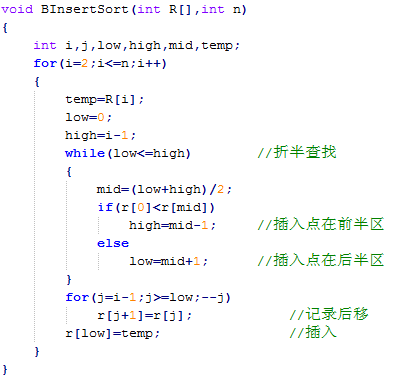
\includegraphics[width=3.70833in,height=3.44792in]{png-jpeg-pics/BD1A9E6E13C293732C4D20448C4FAC01.png}

算法分析:折半插入排序的比较次数比直接插入排序的少,而移动次数相同,\textbf{{因此,总的时间复杂度仍为}{O(n}\textsuperscript{{2}}{)}},另外,折半插入排序也是一种稳定的排序方法。
